\documentclass{article}\usepackage[]{graphicx}\usepackage[]{color}
%% maxwidth is the original width if it is less than linewidth
%% otherwise use linewidth (to make sure the graphics do not exceed the margin)
\makeatletter
\def\maxwidth{ %
  \ifdim\Gin@nat@width>\linewidth
    \linewidth
  \else
    \Gin@nat@width
  \fi
}
\makeatother

\definecolor{fgcolor}{rgb}{0.345, 0.345, 0.345}
\newcommand{\hlnum}[1]{\textcolor[rgb]{0.686,0.059,0.569}{#1}}%
\newcommand{\hlstr}[1]{\textcolor[rgb]{0.192,0.494,0.8}{#1}}%
\newcommand{\hlcom}[1]{\textcolor[rgb]{0.678,0.584,0.686}{\textit{#1}}}%
\newcommand{\hlopt}[1]{\textcolor[rgb]{0,0,0}{#1}}%
\newcommand{\hlstd}[1]{\textcolor[rgb]{0.345,0.345,0.345}{#1}}%
\newcommand{\hlkwa}[1]{\textcolor[rgb]{0.161,0.373,0.58}{\textbf{#1}}}%
\newcommand{\hlkwb}[1]{\textcolor[rgb]{0.69,0.353,0.396}{#1}}%
\newcommand{\hlkwc}[1]{\textcolor[rgb]{0.333,0.667,0.333}{#1}}%
\newcommand{\hlkwd}[1]{\textcolor[rgb]{0.737,0.353,0.396}{\textbf{#1}}}%

\usepackage{framed}
\makeatletter
\newenvironment{kframe}{%
 \def\at@end@of@kframe{}%
 \ifinner\ifhmode%
  \def\at@end@of@kframe{\end{minipage}}%
  \begin{minipage}{\columnwidth}%
 \fi\fi%
 \def\FrameCommand##1{\hskip\@totalleftmargin \hskip-\fboxsep
 \colorbox{shadecolor}{##1}\hskip-\fboxsep
     % There is no \\@totalrightmargin, so:
     \hskip-\linewidth \hskip-\@totalleftmargin \hskip\columnwidth}%
 \MakeFramed {\advance\hsize-\width
   \@totalleftmargin\z@ \linewidth\hsize
   \@setminipage}}%
 {\par\unskip\endMakeFramed%
 \at@end@of@kframe}
\makeatother

\definecolor{shadecolor}{rgb}{.97, .97, .97}
\definecolor{messagecolor}{rgb}{0, 0, 0}
\definecolor{warningcolor}{rgb}{1, 0, 1}
\definecolor{errorcolor}{rgb}{1, 0, 0}
\newenvironment{knitrout}{}{} % an empty environment to be redefined in TeX

\usepackage{alltt}
\usepackage{fullpage}
\usepackage[colorlinks=true,linkcolor=blue]{hyperref}
\title{STAT 675 HW \#4}
\author{Dominic D LaRoche}
\IfFileExists{upquote.sty}{\usepackage{upquote}}{}
\begin{document}
\maketitle

\begin{itemize}
\item[9.1] Repeat example 9.1.\\

\begin{knitrout}
\definecolor{shadecolor}{rgb}{0.969, 0.969, 0.969}\color{fgcolor}\begin{kframe}
\begin{alltt}
\hlkwd{set.seed}(36)
f <- \hlkwd{function}(x, sigma) \{
    \hlkwd{if} (\hlkwd{any}(x < 0)) 
        \hlkwd{return}(0)
    \hlkwd{stopifnot}(sigma > 0)
    \hlkwd{return}((x/sigma^2) * \hlkwd{exp}(-x^2/(2 * sigma^2)))
\}

m <- 10000
sigma <- 2  \hlcom{#changed to sigma=2}
x <- \hlkwd{numeric}(m)
x[1] <- \hlkwd{rchisq}(1, df = 1)
k <- 0
u <- \hlkwd{runif}(m)

\hlkwd{for} (i in 2:m) \{
    xt <- x[i - 1]
    y <- \hlkwd{rchisq}(1, df = xt)
    num <- \hlkwd{f}(y, sigma) * \hlkwd{dchisq}(xt, df = y)
    den <- \hlkwd{f}(xt, sigma) * \hlkwd{dchisq}(y, df = xt)
    \hlkwd{if} (u[i] <= num/den) 
        x[i] <- y else \{
        x[i] <- xt
        k <- k + 1  \hlcom{#y is rejected}
    \}
\}

k
\end{alltt}
\begin{verbatim}
## [1] 5297
\end{verbatim}
\begin{alltt}

reject <- 100 * (k/m)
reject
\end{alltt}
\begin{verbatim}
## [1] 52.97
\end{verbatim}
\begin{alltt}

index <- 5000:5500
y1 <- x[index]
\hlkwd{par}(mfrow = \hlkwd{c}(2, 1))
\hlkwd{plot}(x, type = \hlstr{"l"}, main = \hlstr{""}, ylab = \hlstr{"x"})
\hlkwd{plot}(index, y1, type = \hlstr{"l"}, main = \hlstr{""}, ylab = \hlstr{"x"})
\end{alltt}
\end{kframe}
\includegraphics[width=\maxwidth]{figure/nine1} 
\begin{kframe}\begin{alltt}
\hlkwd{par}(mfrow = \hlkwd{c}(1, 1))
\end{alltt}
\end{kframe}
\end{knitrout}

Compared to example 9.1 this sampler is even more inefficient with a rejection rate of 53\% as opposed to 40\%.  This higher rejection rate is clear in the zoomed in plot in which one can see that the value of x gets stuck for longer periods of time leading to poor mixing of the chain.\\

\item[9.2]  Repeat example 9.1 with gamma($X_t$,1) proposal distribution.\\

\begin{knitrout}
\definecolor{shadecolor}{rgb}{0.969, 0.969, 0.969}\color{fgcolor}\begin{kframe}
\begin{alltt}
\hlkwd{set.seed}(36)
f <- \hlkwd{function}(x, sigma) \{
    \hlkwd{if} (\hlkwd{any}(x < 0)) 
        \hlkwd{return}(0)
    \hlkwd{stopifnot}(sigma > 0)
    \hlkwd{return}((x/sigma^2) * \hlkwd{exp}(-x^2/(2 * sigma^2)))
\}

m <- 10000
sigma <- 4  \hlcom{#changed back to sigma=4}
x <- \hlkwd{numeric}(m)
x[1] <- \hlkwd{rgamma}(1, shape = 1, rate = 1)
k <- 0
u <- \hlkwd{runif}(m)

\hlkwd{for} (i in 2:m) \{
    xt <- x[i - 1]
    y <- \hlkwd{rgamma}(1, shape = xt, rate = 1)
    num <- \hlkwd{f}(y, sigma) * \hlkwd{dgamma}(xt, shape = y, rate = 1)
    den <- \hlkwd{f}(xt, sigma) * \hlkwd{dgamma}(y, shape = xt, rate = 1)
    \hlkwd{if} (u[i] <= num/den) 
        x[i] <- y else \{
        x[i] <- xt
        k <- k + 1  \hlcom{#y is rejected}
    \}
\}

k
\end{alltt}
\begin{verbatim}
## [1] 2873
\end{verbatim}
\begin{alltt}

reject <- 100 * (k/m)
reject
\end{alltt}
\begin{verbatim}
## [1] 28.73
\end{verbatim}
\begin{alltt}

index <- 5000:5500
y1 <- x[index]
\hlkwd{par}(mfrow = \hlkwd{c}(2, 1))
\hlkwd{plot}(x, type = \hlstr{"l"}, main = \hlstr{""}, ylab = \hlstr{"x"})
\hlkwd{plot}(index, y1, type = \hlstr{"l"}, main = \hlstr{""}, ylab = \hlstr{"x"})
\end{alltt}
\end{kframe}
\includegraphics[width=\maxwidth]{figure/nine2} 
\begin{kframe}\begin{alltt}
\hlkwd{par}(mfrow = \hlkwd{c}(1, 1))
\end{alltt}
\end{kframe}
\end{knitrout}

This plot shows better mixing than than the Rayleigh with sigma=2 and has a lower rejection rate than the $\chi^2$ version.\\

\item[9.3] Useing Metropolis-Hastings sampler to generate a sntandard Cauchy

\begin{knitrout}
\definecolor{shadecolor}{rgb}{0.969, 0.969, 0.969}\color{fgcolor}\begin{kframe}
\begin{alltt}
\hlkwd{set.seed}(36)
f <- \hlkwd{function}(x, theta, eta) \{
    \hlkwd{stopifnot}(theta > 0)
    \hlkwd{return}(1/(theta * pi * (1 + ((x - eta)/theta)^2)))
\}
m <- 1e+05
theta <- 1
eta <- 0
x <- \hlkwd{numeric}(m)
x[1] <- \hlkwd{rnorm}(1)  \hlcom{#use the standard normal to start.}
k <- 0
u <- \hlkwd{runif}(m)
\hlkwd{for} (i in 2:m) \{
    xt <- x[i - 1]
    y <- \hlkwd{rnorm}(1, mean = xt, sd = 1)
    num <- \hlkwd{f}(y, theta, eta)
    den <- \hlkwd{f}(xt, theta, eta)  \hlcom{# * \hlkwd{dnorm}(y, mean = xt, sd=1) it cancels out}
    \hlkwd{if} (u[i] <= num/den) 
        x[i] <- y else \{
        x[i] <- xt
        k <- k + 1  \hlcom{#y is rejected}
    \}
\}
k
\end{alltt}
\begin{verbatim}
## [1] 22252
\end{verbatim}
\begin{alltt}
reject <- 100 * (k/m)
reject
\end{alltt}
\begin{verbatim}
## [1] 22.25
\end{verbatim}
\begin{alltt}
index <- 5000:5500
y1 <- x[index]
\hlkwd{par}(mfrow = \hlkwd{c}(2, 1))
\hlkwd{plot}(x, type = \hlstr{"l"}, main = \hlstr{""}, ylab = \hlstr{"x"})
\hlkwd{plot}(index, y1, type = \hlstr{"l"}, main = \hlstr{""}, ylab = \hlstr{"x"})
\end{alltt}
\end{kframe}
\includegraphics[width=\maxwidth]{figure/nine3} 
\begin{kframe}\begin{alltt}
\hlkwd{par}(mfrow = \hlkwd{c}(1, 1))

c <- x[1001:\hlkwd{length}(x)]
q1 <- \hlkwd{quantile}(c, \hlkwd{seq}(0.1, 0.9, 0.1))
q2 <- \hlkwd{qcauchy}(\hlkwd{seq}(0.1, 0.9, 0.1))
q.compare <- \hlkwd{rbind}(q1, q2)
\hlkwd{rownames}(q.compare) <- \hlkwd{c}(\hlstr{"From Sampler"}, \hlstr{"Theoretical"})
\end{alltt}
\end{kframe}
\end{knitrout}

I am not impressed with the approximation of this sample to the theoretical deciles.\\

\item[9.4]  Random walk Metropolis for Laplace distribution.\\

Using modified code from the book's website:\\
\begin{knitrout}
\definecolor{shadecolor}{rgb}{0.969, 0.969, 0.969}\color{fgcolor}\begin{kframe}
\begin{alltt}
\hlkwd{set.seed}(36)
dl <- \hlkwd{function}(x) \{
    0.5 * \hlkwd{exp}(-\hlkwd{abs}(x))
\}  \hlcom{#Standard laplace pdf}

rw.Metropolis.l <- \hlkwd{function}(sigma, x0, N) \{
    x <- \hlkwd{numeric}(N)
    x[1] <- x0
    u <- \hlkwd{runif}(N)
    k <- 0
    \hlkwd{for} (i in 2:N) \{
        y <- \hlkwd{rnorm}(1, x[i - 1], sigma)
        \hlkwd{if} (u[i] <= (\hlkwd{dl}(y)/\hlkwd{dl}(x[i - 1]))) 
            x[i] <- y else \{
            x[i] <- x[i - 1]
            k <- k + 1
        \}
    \}
    \hlkwd{return}(\hlkwd{list}(x = x, k = k))
\}

N <- 10000
sigma <- \hlkwd{c}(0.05, 0.5, 2, 16)
x0 <- 25
rw1 <- \hlkwd{rw.Metropolis.l}(sigma[1], x0, N)
rw2 <- \hlkwd{rw.Metropolis.l}(sigma[2], x0, N)
rw3 <- \hlkwd{rw.Metropolis.l}(sigma[3], x0, N)
rw4 <- \hlkwd{rw.Metropolis.l}(sigma[4], x0, N)


\hlkwd{par}(mfrow = \hlkwd{c}(2, 2))
\hlkwd{plot}(rw1$x, type = \hlstr{"l"}, main = \hlstr{""}, ylab = \hlstr{"x1, sigma=0.05"})
\hlkwd{plot}(rw2$x, type = \hlstr{"l"}, main = \hlstr{""}, ylab = \hlstr{"x2, sigma=0.5"})
\hlkwd{plot}(rw3$x, type = \hlstr{"l"}, main = \hlstr{""}, ylab = \hlstr{"x3, sigma=2"})
\hlkwd{plot}(rw4$x, type = \hlstr{"l"}, main = \hlstr{""}, ylab = \hlstr{"x4,sigma=16"})
\end{alltt}
\end{kframe}
\includegraphics[width=\maxwidth]{figure/nine4} 
\begin{kframe}\begin{alltt}
\hlkwd{par}(mfrow = \hlkwd{c}(1, 1))
\end{alltt}
\end{kframe}
\end{knitrout}

\begin{knitrout}
\definecolor{shadecolor}{rgb}{0.969, 0.969, 0.969}\color{fgcolor}\begin{kframe}
\begin{alltt}
\hlcom{# acceptnce rate}
\hlkwd{print}(\hlkwd{c}(1 - (rw1$k/N), 1 - (rw2$k/N), 1 - (rw3$k/N), 1 - (rw4$k/N)))
\end{alltt}
\begin{verbatim}
## [1] 0.9815 0.8330 0.5291 0.0989
\end{verbatim}
\end{kframe}
\end{knitrout}

Only the chain with sigma=2 has the acceptance rate in the range recommended by the book.  The mixing of the chain for sigma=2 also appears to tbe the best.\\

\item[9.6]  Posterior distribution of the multinomial distribution with probabilities,
$$\frac{\left(\frac{1}{2}+\frac{\theta}{4},\frac{1-\theta}{4},\frac{1-\theta}{4},\frac{\theta}{4}\right)}{x_1!x_2!x_3!x_4!}$$
I will use the metropolis-hastings sampler with the uniform(0,1) as the prior (per request in the HW assignment) and implement with modified code from the book.  The posterior density is proportional to:
$$f(X|\theta) = \frac{\pi(\theta)f(Y|\theta)}{f(Y)} \propto 1 \times p_1 \times p_2 \times p_3 \times p_4$$
which in this case is :\\
$$\left(\frac{2+Y}{4}\right)^{x_1}\left(\frac{1-Y}{4}\right)^{x_2+x_3}\left(\frac{Y}{4}\right)^{x_4}$$


\begin{knitrout}
\definecolor{shadecolor}{rgb}{0.969, 0.969, 0.969}\color{fgcolor}\begin{kframe}
\begin{alltt}
m <- 10000  \hlcom{#length of the chain}

burn <- 1000  \hlcom{#burn-in time}
animals <- 197
x <- \hlkwd{numeric}(m)  \hlcom{#the chain}

\hlcom{# the observed frequencies of x}
xfreq <- \hlkwd{c}(125, 18, 20, 34)

prob <- \hlkwd{function}(theta, x) \{
\hlcom{    # computes (without the constants which cancel) the target density}
    \hlkwd{if} (theta < 0 || theta > 1) \{
\hlcom{        #bound on theta}
        \hlkwd{return}(0)
    \} else \{
        p <- (2 + theta)^x[1] * (1 - theta)^(x[2] + x[3]) * (theta)^x[4]
        \hlkwd{return}(p)
    \}
\}
\hlkwd{curve}(\hlkwd{prob}(x, xfreq))
\end{alltt}
\end{kframe}
\includegraphics[width=\maxwidth]{figure/nine6} 

\end{knitrout}

The Beta($\alpha,\beta$) has the same support as $\theta$ and I have frequently seen it used to model probabilities so I will use it as the proposal density.  I experimented with various ways to set the parameters of the beta proposal density.  Setting the two shape parameters equal to each other would create symmetric densities centered around .5.  However, since the values of alpha and beta would be \textless 1, the bulk of the dnsity would be close to 0 and 1, which led to a very low acceptance rate.  Multiplying both alpha and beta by a constant to shift the density to the center did not alleviate the problem. Making the beta density assymetric by setting the beta=1 also lead to a very low acceptance rate.  All of the methods arrived at a similar $\hat{\theta}$ estimate of \\

\begin{knitrout}
\definecolor{shadecolor}{rgb}{0.969, 0.969, 0.969}\color{fgcolor}\begin{kframe}
\begin{alltt}
\hlkwd{set.seed}(36)
u <- \hlkwd{runif}(m) \hlcom{#for accept/reject step}
k<-0
x[1] <- .5
\hlkwd{for} (i in 2:m) \{
    y <- \hlkwd{rbeta}(1, x[i-1], 1)  \hlcom{# symmetric proposal distribution}
    
  \hlkwd{if} (u[i] <= (\hlkwd{prob}(y, xfreq)*\hlkwd{dbeta}(x[i-1],y,1)) / (\hlkwd{prob}(x[i-1], xfreq)*\hlkwd{dbeta}(y,x[i-1],1)))\hlcom{#}
    x[i] <- y  else
        x[i] <- x[i-1]
        k <- k+1
\}

\hlkwd{plot}( x, type=\hlstr{"l"}, main=\hlstr{""}, ylab=\hlstr{"x"})
\end{alltt}
\end{kframe}
\includegraphics[width=\maxwidth]{figure/nine62} 
\begin{kframe}\begin{alltt}
\hlcom{#acceptance rate}
1-(k/m)
\end{alltt}
\begin{verbatim}
## [1] 1e-04
\end{verbatim}
\begin{alltt}

xb <- x[(burn+1):m]
th.hat<-\hlkwd{mean}(xb)
\hlkwd{print}(th.hat)
\end{alltt}
\begin{verbatim}
## [1] 0.6232
\end{verbatim}
\begin{alltt}

i <- \hlkwd{sample}(1:4, size=animals, replace=TRUE,prob=\hlkwd{c}((2+th.hat)/4, 
                  (1-th.hat)/4, (1-th.hat)/4, th.hat/4))
predicted <- \hlkwd{tabulate}(i)
\hlkwd{print}(\hlkwd{rbind}(predicted,xfreq))
\end{alltt}
\begin{verbatim}
##           [,1] [,2] [,3] [,4]
## predicted  131   16   20   30
## xfreq      125   18   20   34
\end{verbatim}
\end{kframe}
\end{knitrout}

All of the methods arrived at a similar estimate of $\hat{\theta}=0.62$. The predicted frequencies also matched up pretty well to the observed frequencies.\\

\item[9.7]  Bivariate normal via Gibbs sampling.\\
I will use code modified from the text.
\begin{knitrout}
\definecolor{shadecolor}{rgb}{0.969, 0.969, 0.969}\color{fgcolor}\begin{kframe}
\begin{alltt}
\hlkwd{set.seed}(36)
\hlcom{# initialize constants and parameters}
N <- 1e+05  \hlcom{#length of chain}
burn <- 10000  \hlcom{#burn-in length}
X <- \hlkwd{matrix}(0, N, 2)  \hlcom{#the chain, a bivariate sample}

rho <- 0.9  \hlcom{#correlation}
mu1 <- 0
mu2 <- 0
sigma1 <- 1
sigma2 <- 1
s1 <- \hlkwd{sqrt}(1 - rho^2) * sigma1
s2 <- \hlkwd{sqrt}(1 - rho^2) * sigma2

\hlcom{###### generate the chain #####}

X[1, ] <- \hlkwd{c}(mu1, mu2)  \hlcom{#initialize}

\hlkwd{for} (i in 2:N) \{
    x2 <- X[i - 1, 2]
    m1 <- mu1 + rho * (x2 - mu2) * sigma1/sigma2
    X[i, 1] <- \hlkwd{rnorm}(1, m1, s1)
    x1 <- X[i, 1]
    m2 <- mu2 + rho * (x1 - mu1) * sigma2/sigma1
    X[i, 2] <- \hlkwd{rnorm}(1, m2, s2)
\}

b <- burn + 1
x <- X[b:N, ]

\hlcom{# compare sample statistics to parameters}
\hlkwd{colMeans}(x)
\end{alltt}
\begin{verbatim}
## [1] -0.004358 -0.003612
\end{verbatim}
\begin{alltt}
\hlkwd{cov}(x)
\end{alltt}
\begin{verbatim}
##        [,1]   [,2]
## [1,] 0.9830 0.8851
## [2,] 0.8851 0.9871
\end{verbatim}
\begin{alltt}
\hlkwd{cor}(x)
\end{alltt}
\begin{verbatim}
##        [,1]   [,2]
## [1,] 1.0000 0.8986
## [2,] 0.8986 1.0000
\end{verbatim}
\begin{alltt}

\hlkwd{plot}(x, main = \hlstr{""}, cex = 0.5, xlab = \hlkwd{bquote}(X[1]), ylab = \hlkwd{bquote}(X[2]), ylim = \hlkwd{range}(x[, 
    2]))
\end{alltt}
\end{kframe}
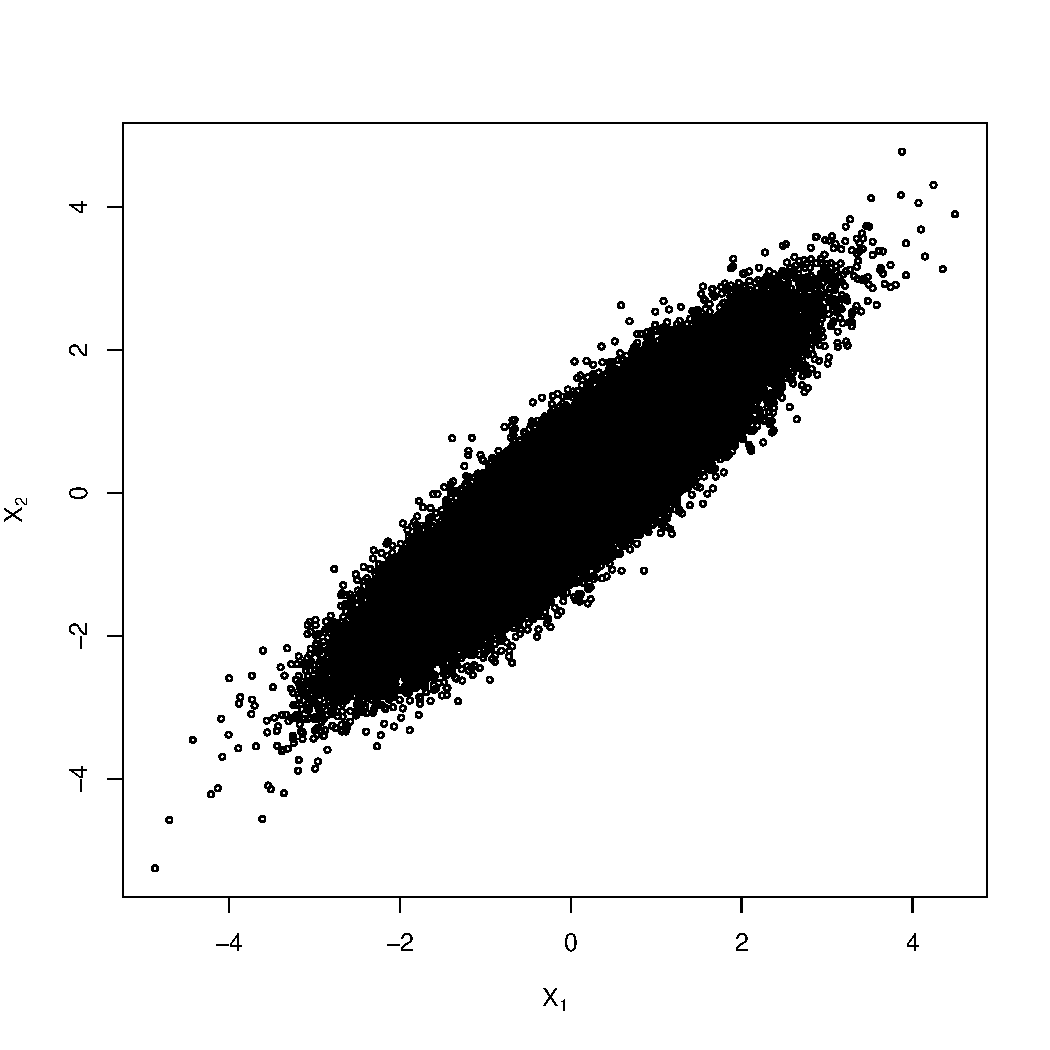
\includegraphics[width=\maxwidth]{figure/nine7} 

\end{knitrout}

The sample statistics compare favorably with the parameters.\\

\item[9.8]  Gibbs sampler with Binomial and Beta conditional distributions.\\

The chain is generated by sampling from the two marginal densities; Binomial($n,y$) and Beta($x+a$, $n-x+b$).  In this case I will use a=2, b=3, and n=10.\\

\begin{knitrout}
\definecolor{shadecolor}{rgb}{0.969, 0.969, 0.969}\color{fgcolor}\begin{kframe}
\begin{alltt}
\hlkwd{set.seed}(36)
\hlcom{# initialize constants and parameters}
N <- 1e+05  \hlcom{#length of chain}
burn <- 10000  \hlcom{#burn-in length}
V <- \hlkwd{matrix}(0, N, 2)  \hlcom{#the chain, a bivariate sample}

a <- 2  \hlcom{#correlation}
b <- 3
n <- 10
y <- 0.5
x <- 0.5

\hlcom{###### generate the chain #####}

V[1, ] <- \hlkwd{c}(y, x)  \hlcom{#initialize}

\hlkwd{for} (i in 2:N) \{
    y1 <- V[i - 1, 2]
    V[i, 1] <- \hlkwd{rbinom}(1, size = n, prob = y1)
    
    x1 <- V[i, 1]
    shape1 <- x1 + a
    shape2 <- n - x1 + b
    V[i, 2] <- \hlkwd{rbeta}(1, shape1, shape2)
\}

b <- burn + 1
v <- V[b:N, ]

\hlkwd{plot}(v, main = \hlstr{""}, cex = 0.5, xlab = y, ylab = x, ylim = \hlkwd{range}(x[, 2]))
\end{alltt}


{\ttfamily\noindent\bfseries\color{errorcolor}{\#\# Error: incorrect number of dimensions}}\end{kframe}
\end{knitrout}


\item[9.9] Modification of the Gelmin-Rubin Convgergence monitor.\\

Using code from the book.
\begin{knitrout}
\definecolor{shadecolor}{rgb}{0.969, 0.969, 0.969}\color{fgcolor}\begin{kframe}
\begin{alltt}
\hlkwd{set.seed}(36)
Gelman.Rubin <- \hlkwd{function}(psi) \{
\hlcom{    # psi[i,j] is the statistic psi(X[i,1:j]) for chain in i-th row of X}
    psi <- \hlkwd{as.matrix}(psi)
    n <- \hlkwd{ncol}(psi)
    k <- \hlkwd{nrow}(psi)
    psi.means <- \hlkwd{rowMeans}(psi)  \hlcom{#row means}
    B <- n * \hlkwd{var}(psi.means)  \hlcom{#between variance est.}
    psi.w <- \hlkwd{apply}(psi, 1, \hlstr{"var"})  #within variances
    W <- \hlkwd{mean}(psi.w)  \hlcom{#within est.}
    v.hat <- W * (n - 1)/n + (B/n)  \hlcom{#upper variance est.}
    r.hat <- v.hat/W  \hlcom{#G-R statistic}
    \hlkwd{return}(r.hat)
\}

normal.chain <- \hlkwd{function}(sigma, N, X1) \{
\hlcom{    # generates a Metropolis chain for Normal(0,1) with Normal(X[t], sigma)}
\hlcom{    # proposal distribution and starting value X1}
    x <- \hlkwd{rep}(0, N)
    x[1] <- X1
    u <- \hlkwd{runif}(N)
    
    \hlkwd{for} (i in 2:N) \{
        xt <- x[i - 1]
        y <- \hlkwd{rnorm}(1, xt, sigma)  \hlcom{#candidate point}
        r1 <- \hlkwd{dnorm}(y, 0, 1) * \hlkwd{dnorm}(xt, y, sigma)
        r2 <- \hlkwd{dnorm}(xt, 0, 1) * \hlkwd{dnorm}(y, xt, sigma)
        r <- r1/r2
        \hlkwd{if} (u[i] <= r) 
            x[i] <- y else x[i] <- xt
    \}
    \hlkwd{return}(x)
\}

sigma <- 0.2  \hlcom{#parameter of proposal distribution}
k <- 4  \hlcom{#number of chains to generate}
n <- 15000  \hlcom{#length of chains}
b <- 1000  \hlcom{#burn-in length}

\hlcom{# choose overdispersed initial values}
x0 <- \hlkwd{c}(-10, -5, 5, 10)
\hlcom{# generate the chains}
X <- \hlkwd{matrix}(0, nrow = k, ncol = n)
\hlkwd{for} (i in 1:k) X[i, ] <- \hlkwd{normal.chain}(sigma, n, x0[i])

\hlcom{# compute diagnostic statistics}
psi <- \hlkwd{t}(\hlkwd{apply}(X, 1, cumsum))
\hlkwd{for} (i in 1:\hlkwd{nrow}(psi)) psi[i, ] <- psi[i, ]/(1:\hlkwd{ncol}(psi))
\hlkwd{print}(\hlkwd{Gelman.Rubin}(psi))
\end{alltt}
\begin{verbatim}
## [1] 1.172
\end{verbatim}
\end{kframe}
\end{knitrout}



\end{itemize}
\end{document}
